\subsubsection*{Project progress \& future work}
\paragraph{Computational model}
The computational modelling work so far had been done using Fusion 360 (Autodesk), but it had limited capabilities on prescribing the needed periodic displacements.
This has led to the usage of Abaqus FEA (Dassault Systèmes) and learning an entirely new workflow.
Progression has been steady albeit slow. Some key sections have been done so far:
\begin{enumerate}
    \item Modal analysis of an ITAP both with and without a flange. This is intended to find resonant frequencies for the type of behaviour (i.e. pattern of the displacement) we want.
    \item One particular frequency-displacement combination
\end{enumerate}

\begin{figure}[h] \centering
    \begin{subfigure}{0.45\textwidth}
        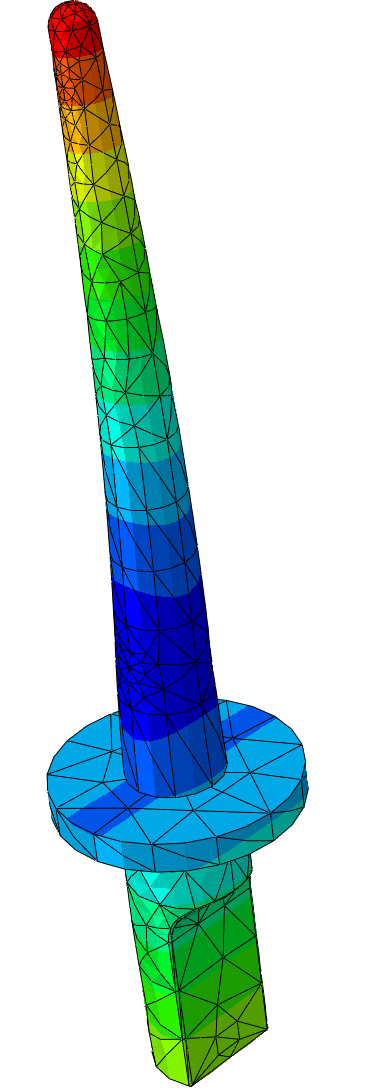
\includegraphics[width=3cm]{figures/model-modal.PNG}
        \caption{}
    \end{subfigure}
    \begin{subfigure}{0.45\textwidth}
        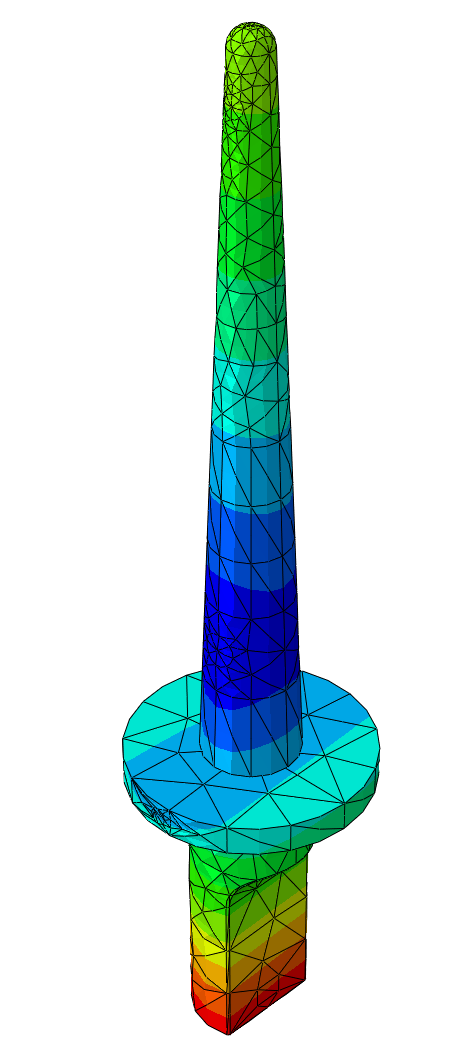
\includegraphics[width=4cm]{figures/model-periodic-displacement.png}
        \caption{}
    \end{subfigure}
    \caption{Computational modeling examples. (a) is the type of visualisation we get from modal analysis. (b) shows the distribution of displacements after some periodic displacement at the base. Scales purposefully omitted because they require more context to be meaningful.}
\end{figure}

The current and future work is in a) automating the production and simulation of displacements and frequencies of clinical revelance (i.e. about \SI{200}{Hz}, far below the first resonance at about \SI{900}{Hz}); b) Get the Abaqus model to the level of detail as the Fusion 360 one; and c) fully cover the spectrum of our dependent and independent variables, described in Table \ref{tb:variables}.
\begin{table}[h]
\centering
\begin{tabular}{cc}
    \textbf{Independent} & \textbf{Dependent} \\ \hline
    Axis of displacement (source) & Magnitude of total displacement (areas of interest) \\
    Magnitude displacement (source) & x,y and z displacements (areas of interest) \\
    Frequency &  \\
\end{tabular}
\caption{Key variables in the experiment}
\label{tb:variables}
\end{table}


\paragraph{Prototyping in the lab}
In terms of learning, the project has come reasonably far.
There is a better understanding of the current uses of feedback with prostheses, vibration perception thresholds, context for clinically relevant frequencies and displacements.
In that sense, we are ready to start prototyping, however, I expected to be fully finished with the finite element analysis before going into the laboratory.

The short-term tasks in preparation for lab work are detailed below, as well as Figure \ref{fig:experimental-setup} which shows the expected experimental setup.

\begin{enumerate}
    \item Meet with others currently working with vibrotactile feedback in the same lab.
    \item Get better acquainted with Precision Microdrives haptics and vibration motors, the actuators used in the lab.
\end{enumerate}

There was a conscious decision to remain unaware of the limited hardware available.
The information being produced by the numerical model is expected to be much broader than those validated by the physical model, and gives the opportunity for informed decision on what --- if anything --- to buy.

\begin{figure}[h]
\centering
    
\includegraphics[width=\textwidth]{figures/experimental-setup.png}
\caption{Model of prototyping setup built in Fusion 360}
\label{fig:experimental-setup}
\end{figure}